\documentclass[10pt,letterpaper]{article}
\usepackage{ccn}
\usepackage{pslatex}
\usepackage{apacite}
\usepackage{graphicx}
\usepackage{natbib}
\usepackage{float}
\usepackage{hyperref}
\usepackage{booktabs}
\usepackage{microtype}
\usepackage{xcolor}
\usepackage{amsmath}
\usepackage[labelfont=bf, margin=0.1cm, font=sf, font+=footnotesize, skip=2pt]{caption}
\graphicspath{{../outputs/}}
\setlength{\textfloatsep}{6pt plus 2pt minus 2pt}
\setlength{\floatsep}{5pt plus 2pt minus 2pt}
% checklist answer macros (as in the course-provided NeurIPS 2024 checklist file)
\newcommand{\answerYes}[1][]{\textcolor{blue}{[Yes] #1}}
\newcommand{\answerNo}[1][]{\textcolor{orange}{[No] #1}}
\newcommand{\answerNA}[1][]{\textcolor{gray}{[NA] #1}}

\title{What Missionary Control Left in the Language of Two 1880s isiXhosa Newspapers}

\author{{\large \bf Emmanuel Azubuike (2698752) \quad George Ayensu (2722188) \quad Banele Mkhize (2663814)} \\ University of the Witwatersrand, Johannesburg, South Africa}

\usepackage{pdfpages}
\begin{document}
\maketitle

\section{Abstract}
{\bf \looseness=-1
From 1884 the missionary \emph{Isigidimi sama-Xosa} and the African-owned \emph{Imvo Zabantsundu} ran side by side. Did missionary control change \emph{what} they printed, or \emph{how} they used words? Imvo was not more political: of ten political topics chosen in advance, only parliament differs, and not after correction. Religion, an exploratory topic, differs most: Isigidimi uses it four times as often, also in readers' letters and under the same editor. How political words were used barely differs. Old spelling costs only the African-language tokenizer more. The evidence fits control shaping what the papers printed, not how they wrote.}

\section{Introduction and Background}\label{Intro}
\looseness=-1
\textbf{Where did missionary control leave its trace in the language of the earliest isiXhosa press?} The IsiXhosa Intellectual Traditions archive \citep{schoots2023} lets us ask this. \emph{Isigidimi sama-Xosa} was a missionary paper. \emph{Imvo Zabantsundu} was founded in 1884 by Isigidimi's former editor, J.\,T.~Jabavu, as the first African-owned isiXhosa paper, free ``from any missionary control'' \citep[p.~55]{schoots2023}. After 1884 both papers had African editors, Gqoba and Jabavu \citep[p.~71]{schoots2023b}. Comparing the papers compares control, but also two editors, places and readerships. So we also compare Jabavu with himself: he edited Isigidimi from 1881 to 1884 and Imvo afterwards.

\begin{figure*}[t]
\centering
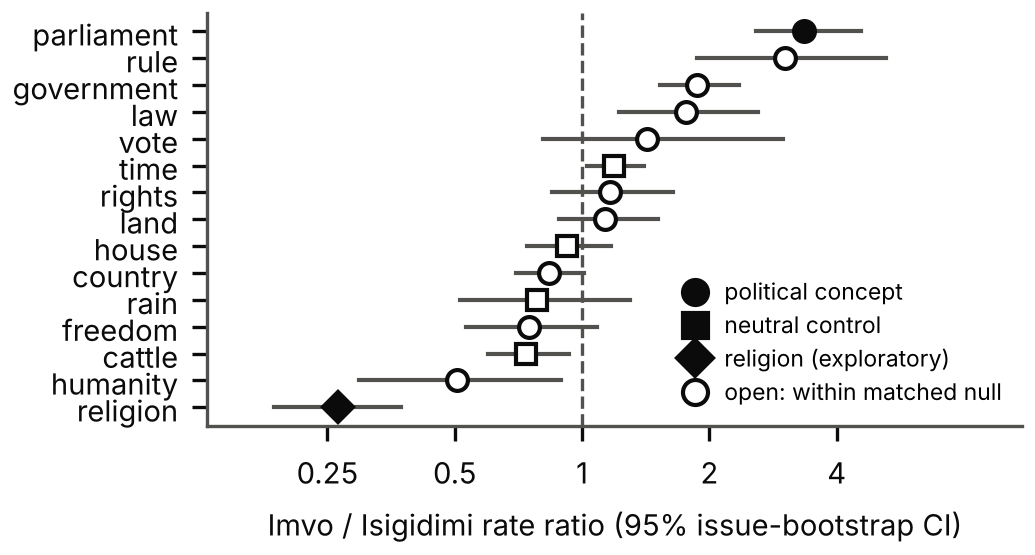
\includegraphics[width=3.0in]{fig_salience.png}\hfill
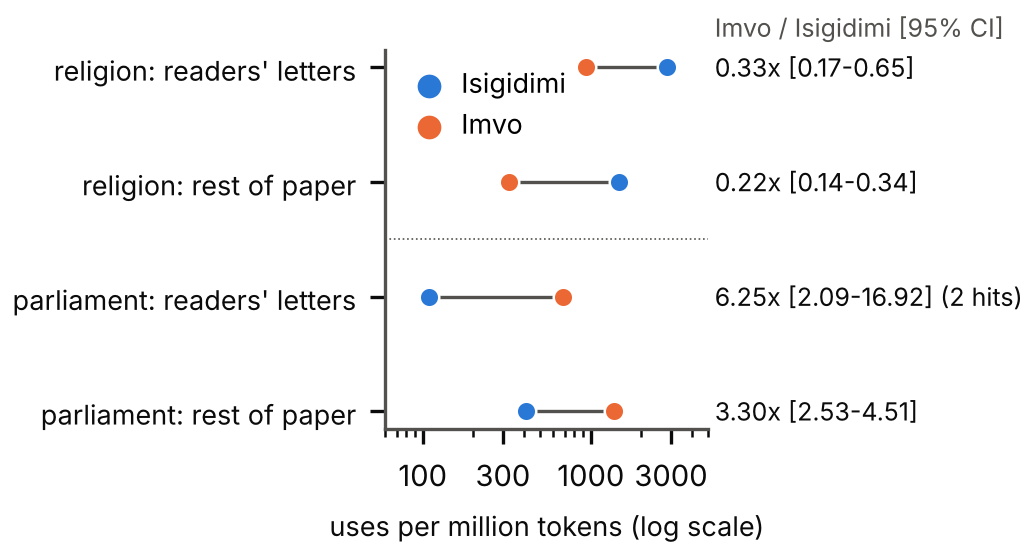
\includegraphics[width=3.15in]{fig_letters.png}
\caption{What the papers printed. Left: how often Imvo uses each topic relative to Isigidimi (ratio with 95\% CI; filled: beats random word sets at $p<0.05$, uncorrected). Right: the religious gap also appears in readers' letters.}
\label{fig:agenda}
\end{figure*}
\begin{figure*}[t]
\centering
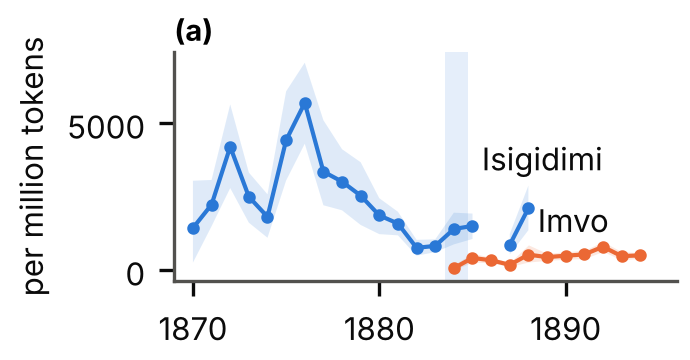
\includegraphics[width=2.1in]{fig_religion_by_year.png}\hfill
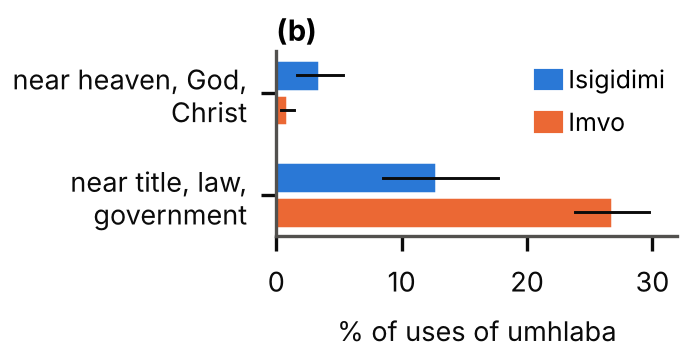
\includegraphics[width=2.1in]{fig_land_senses.png}\hfill
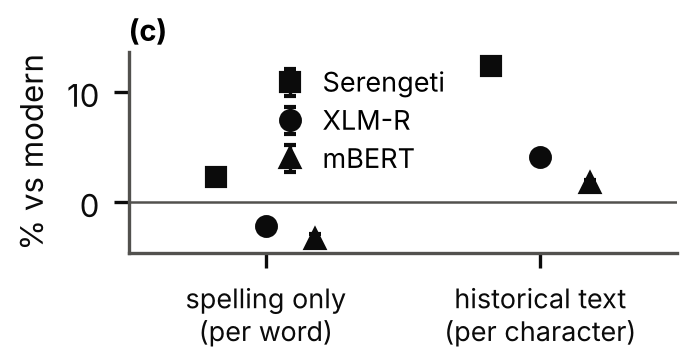
\includegraphics[width=2.1in]{fig_tokenizer_cost.png}
\caption{(a) Religious words per million; grey: years Jabavu edited Isigidimi before moving to Imvo; Gqoba edited Isigidimi from late 1884. (b) How often \emph{umhlaba} appears near religious or legal words (95\% CI). (c) Extra subword pieces compared with modern text (95\% CIs are smaller than the markers).}
\label{fig:how}
\end{figure*}

Communication research distinguishes what a paper covers, \emph{agenda-setting} \citep{mccombs1972}, from how it presents it, \emph{framing} \citep{entman1993}. We measure coverage as \textbf{salience}: how often a topic's words appear. We study framing with word embeddings, which place each word by its neighbours \citep{hamilton2016}. Most such studies use modern news \citep{card2015,field2018}; for these papers, \citet{schoots2023b} counted root words over time. We add controlled comparisons, the same-editor test and a letters-versus-rest split, and ask whether this history still affects how machines read the archive \citep{petrov2023,rust2021}. \textbf{H1}: the papers differ in how often they use political and religious words. \textbf{H2}: Isigidimi uses political words in more religious contexts. \textbf{H3}: old text and spelling cost tokenizers more.

\begin{table}[t]
\centering\footnotesize
\begin{tabular}{@{}p{1.18in}p{2.02in}@{}}
\toprule
\textbf{Threat} & \textbf{Response} \\ \midrule
Different years & Nov 1884--1888 only; month-matched draws \\
Imvo 4.6$\times$ larger & Ten Imvo samples of Isigidimi's size \\
Frequency effects & 2000 matched random word sets \citep{monroe2008} \\
Change over time & Each paper's own drift in other years \\
Unstable embeddings & Tune for seed stability; average ten runs \\
Non-political effects & Four neutral control concepts \\
One paper per side & Same editor in both; place, audience unfixed \\
\bottomrule
\end{tabular}
\caption{Threats to a fair comparison, and our response.}
\label{tab:design}
\end{table}

\section{Methods}
\looseness=-1
\textbf{Data.} We use the archive's human-corrected transcriptions, which were not spell-checked \citep[p.~59]{schoots2023}, from November 1884 to 1888: 286{,}663 words of Isigidimi and 1.31 million of Imvo (safeguards in Table~\ref{tab:design}).

\textbf{Salience.} Each topic is a set of word stems, adapted from \citet{schoots2023b} (Table S1). We fixed ten political topics in advance, plus four neutral controls. Religion (\emph{tixo}, \emph{kristu}) is exploratory: a classifier trained on the same years suggested it (logistic regression, @@CLFACC@@ balanced accuracy; chance 0.50), though the archive's authors also expect it \citep[p.~57]{schoots2023}. We compare rates per million words. Bootstrap confidence intervals test whether the rates differ; matched random word sets ask the stricter question: does it differ more than random words of the same frequency? For the same-editor contrast, Jabavu's Isigidimi runs from January 1881 to October 1884.

\textbf{Letters.} A reader's letter opens by addressing the editor (\emph{nkosi mhleli \dots\ kaundifakele}, `sir, editor \dots\ please print') and ends with a signature. In a hand check, @@LETPREC@@ detected letters were genuine (Table S5).

\textbf{Framing.} Embeddings capture a word's meaning, grammar and topic, so they are only a rough proxy for framing in Entman's sense. We train fastText embeddings \citep{bojanowski2017}, tuning @@NTUNE@@ settings (Table S8) on other years for stability across random seeds, since unstable embeddings create false shifts \citep{antoniak2018}. The chosen narrow window favours grammar, so we also report wider ones. A word's \emph{shift} measures how differently it relates to 500 common words in each paper \citep{hamilton2016b}; shuffling issues between the papers gives the level expected by chance \citep{dubossarsky2017}. A directional test, the part aimed at framing, asks whether political words sit closer to religious or to political words (Table S4). We also count religious and legal words near \emph{umhlaba}.

\textbf{Tokenizers.} We count the subword pieces that XLM-R \citep{conneau2020}, Serengeti \citep{adebara2023} and mBERT \citep{devlin2019} need for modern news \citep{adelani2023}, for the same news in old spelling, and for our historical text.

\section{Results}
\looseness=-1
\textbf{H1: different topics, but not more politics.} Of the ten political topics, only parliament differs: Imvo uses it @@SPAR@@ times as often ($p=@@SPARP@@$; Fig.~\ref{fig:agenda}, left). Law, vote, rights, land and government do not differ. Religion differs most: Isigidimi uses it @@SRELINV@@ times as often ($p=@@SRELP@@$). Neither result survives correction for 15 tests. The religious gap appears in readers' letters as well as in the rest of each paper (Fig.~\ref{fig:agenda}, right). It also holds under one editor: Jabavu's Imvo used religious words a third as often as Jabavu's Isigidimi ($p=@@ECRELP@@$). Under Gqoba, Isigidimi did not fall further ($p=@@EDRELP@@$). Before Imvo existed, Isigidimi's religious words were already falling, while parliament and vote rose sharply (Fig.~\ref{fig:how}a; Table S7).

\textbf{H2: little difference in how words are used.} Overall word use differs (shift @@OBS@@ vs @@NULL@@ by chance), but no topic stands out: parliament shifts no more than the neutral control \emph{cattle} (Fig.~S1). Political words do sit closer to religious words in Isigidimi, in all five settings and in three after correction (Table S2). But this depends on one word, \emph{land} (\emph{umhlaba}), and the neutral control \emph{house} shows the same lean@@ENDLUSENT@@. The papers also use \emph{umhlaba} differently: Isigidimi puts it near religious words in @@LSRI@@\% of uses, Imvo in @@LSRM@@\% (Fig.~\ref{fig:how}b). Finally, a single word must shift by @@FLOOR1@@ to be detected, more than the whole gap between the papers (@@GAP1@@).

\textbf{H3: historical text costs more.} Our historical text needs @@SHI@@\%, @@XHI@@\% and @@MHI@@\% more subword pieces per character with Serengeti, XLM-R and mBERT; old spelling alone raises only Serengeti's cost (Fig.~\ref{fig:how}c).

\section{Discussion}
\looseness=-1
\textbf{Is it control, or just time? (H1).} Religious words were falling in Isigidimi anyway, so we combine two comparisons with different blind spots. Imvo against Gqoba's Isigidimi holds the years fixed; Jabavu's two papers hold the editor fixed. Both show the gap, and the second uses years the classifier never saw, partly replicating the religion finding. If the gap were only the falling trend, Isigidimi would have kept falling after 1884; it did not. Had Jabavu's Imvo been as religious as his Isigidimi, control would be refuted; it was not. The argument rests on these two comparisons agreeing, not on their uncorrected $p$-values. We cannot say whether Jabavu was right to leave; leaving brought less religion, not clearly more politics.

The gap is not only the editors' voice, or the sections each paper ran. Isigidimi's letter-writers used religious words three times as often as Imvo's, so each paper drew on, or chose, different writers. One wrote to Isigidimi: \emph{ilizwi alizanga ukuba silipate, lize ukuba lisipate} (`the Word did not come for us to carry it; it came to carry [or rule] us'; 1884; our gloss).

\textbf{What the embeddings show (H2).} The framing signal looks like a difference in meaning, not slant: Isigidimi more often uses \emph{umhlaba} for the earth, Imvo for land under law, which alone would move the word in each model. The detection floor rules out large framing differences, but not small ones.

\textbf{Responsible NLP (H3).} This history still affects today's tools: written isiXhosa took shape in the mission press (cf.\ \citealp{gilmour2007}), and its old spelling penalises only the model built for African languages. Serengeti's vocabulary has twice XLM-R's share of \emph{th}, \emph{kh} and \emph{ph} pieces (@@SERTH@@\% vs @@XLMTH@@\%), which may explain this. A modern-spelling copy can help tools but must not replace the original, as the conversion loses information (old \emph{t} can be \emph{t} or \emph{th}). We describe two papers, not isiXhosa speakers; cultural claims without speakers' review would be extractive \citep{bird2020}.

\textbf{Limitations and conclusion.} Two papers, one period, a missing year, an incomplete editor comparison, an automatic letter split, unreviewed translations. Still, the evidence fits control shaping what the papers printed, letters included; any effect on how they wrote is too small to detect.

\bibliographystyle{apacite}
\setlength{\bibleftmargin}{.125in}
\setlength{\bibindent}{-\bibleftmargin}
\bibliography{paper}

\clearpage
\onecolumn
\small
\section*{NeurIPS Paper Checklist}
\begin{enumerate}

\item {\bf Claims}
    \item[] Question: Do the main claims made in the abstract and introduction accurately reflect the paper's contributions and scope?
    \item[] Answer: \answerYes{}
    \item[] Justification: The abstract and introduction state three hypotheses (H1 salience, H2 framing, H3 tokenizer cost) and report what was found: of ten pre-specified political concepts only parliament differs (uncorrected); the exploratory religious gap holds in readers' letters, in the same years and under the same editor (Jabavu), while the editor change within Isigidimi is not distinguishable from random words; political vocabulary followed the times; and the negative results (framing is weak and non-specific; the directional lean survives correction in three of five settings, but in at most one without land, and a neutral control leans further; the lean rests on umhlaba, which the two papers use in different senses). Claims about meaning are scoped as unreviewed by a first-language speaker.
    \item[] Guidelines:
    \begin{itemize}
        \item The answer NA means that the abstract and introduction do not include the claims made in the paper.
        \item The abstract and/or introduction should clearly state the claims made, including the contributions made in the paper and important assumptions and limitations. A No or NA answer to this question will not be perceived well by the reviewers. 
        \item The claims made should match theoretical and experimental results, and reflect how much the results can be expected to generalize to other settings. 
        \item It is fine to include aspirational goals as motivation as long as it is clear that these goals are not attained by the paper. 
    \end{itemize}

\item {\bf Limitations}
    \item[] Question: Does the paper discuss the limitations of the work performed by the authors?
    \item[] Answer: \answerYes{}
    \item[] Justification: The Discussion ends with limitations (two newspapers, one window, 1886 Isigidimi editions missing, an incomplete control-by-editor design, a heuristic letter split, a modern-news domain mismatch, unreviewed stems and glosses; the Results flag the one-model tokenizer hypothesis, and Table S3 the era-confounded held-out windows) and states the detection floor of the framing test.
    \item[] Guidelines:
    \begin{itemize}
        \item The answer NA means that the paper has no limitation while the answer No means that the paper has limitations, but those are not discussed in the paper. 
        \item The authors are encouraged to create a separate "Limitations" section in their paper.
        \item The paper should point out any strong assumptions and how robust the results are to violations of these assumptions (e.g., independence assumptions, noiseless settings, model well-specification, asymptotic approximations only holding locally). The authors should reflect on how these assumptions might be violated in practice and what the implications would be.
        \item The authors should reflect on the scope of the claims made, e.g., if the approach was only tested on a few datasets or with a few runs. In general, empirical results often depend on implicit assumptions, which should be articulated.
        \item The authors should reflect on the factors that influence the performance of the approach. For example, a facial recognition algorithm may perform poorly when image resolution is low or images are taken in low lighting. Or a speech-to-text system might not be used reliably to provide closed captions for online lectures because it fails to handle technical jargon.
        \item The authors should discuss the computational efficiency of the proposed algorithms and how they scale with dataset size.
        \item If applicable, the authors should discuss possible limitations of their approach to address problems of privacy and fairness.
        \item While the authors might fear that complete honesty about limitations might be used by reviewers as grounds for rejection, a worse outcome might be that reviewers discover limitations that aren't acknowledged in the paper. The authors should use their best judgment and recognize that individual actions in favor of transparency play an important role in developing norms that preserve the integrity of the community. Reviewers will be specifically instructed to not penalize honesty concerning limitations.
    \end{itemize}

\item {\bf Theory Assumptions and Proofs}
    \item[] Question: For each theoretical result, does the paper provide the full set of assumptions and a complete (and correct) proof?
    \item[] Answer: \answerNA{}
    \item[] Justification: The paper has no theoretical results.
    \item[] Guidelines:
    \begin{itemize}
        \item The answer NA means that the paper does not include theoretical results. 
        \item All the theorems, formulas, and proofs in the paper should be numbered and cross-referenced.
        \item All assumptions should be clearly stated or referenced in the statement of any theorems.
        \item The proofs can either appear in the main paper or the supplemental material, but if they appear in the supplemental material, the authors are encouraged to provide a short proof sketch to provide intuition. 
        \item Inversely, any informal proof provided in the core of the paper should be complemented by formal proofs provided in appendix or supplemental material.
        \item Theorems and Lemmas that the proof relies upon should be properly referenced. 
    \end{itemize}

    \item {\bf Experimental Result Reproducibility}
    \item[] Question: Does the paper fully disclose all the information needed to reproduce the main experimental results of the paper to the extent that it affects the main claims and/or conclusions of the paper (regardless of whether the code and data are provided or not)?
    \item[] Answer: \answerYes{}
    \item[] Justification: The Methods give the window, the date-matched subsampling, concept stems, model and hyper-parameter choices, the permutation null, the matched-set tests and the tokenizer conditions. Anchor lists are summarised in Table S4; word-joining and tokenizer rewrite rules are in the submitted code and README.txt, which gives the run order; seeds are fixed.
    \item[] Guidelines:
    \begin{itemize}
        \item The answer NA means that the paper does not include experiments.
        \item If the paper includes experiments, a No answer to this question will not be perceived well by the reviewers: Making the paper reproducible is important, regardless of whether the code and data are provided or not.
        \item If the contribution is a dataset and/or model, the authors should describe the steps taken to make their results reproducible or verifiable. 
        \item Depending on the contribution, reproducibility can be accomplished in various ways. For example, if the contribution is a novel architecture, describing the architecture fully might suffice, or if the contribution is a specific model and empirical evaluation, it may be necessary to either make it possible for others to replicate the model with the same dataset, or provide access to the model. In general. releasing code and data is often one good way to accomplish this, but reproducibility can also be provided via detailed instructions for how to replicate the results, access to a hosted model (e.g., in the case of a large language model), releasing of a model checkpoint, or other means that are appropriate to the research performed.
        \item While NeurIPS does not require releasing code, the conference does require all submissions to provide some reasonable avenue for reproducibility, which may depend on the nature of the contribution. For example
        \begin{enumerate}
            \item If the contribution is primarily a new algorithm, the paper should make it clear how to reproduce that algorithm.
            \item If the contribution is primarily a new model architecture, the paper should describe the architecture clearly and fully.
            \item If the contribution is a new model (e.g., a large language model), then there should either be a way to access this model for reproducing the results or a way to reproduce the model (e.g., with an open-source dataset or instructions for how to construct the dataset).
            \item We recognize that reproducibility may be tricky in some cases, in which case authors are welcome to describe the particular way they provide for reproducibility. In the case of closed-source models, it may be that access to the model is limited in some way (e.g., to registered users), but it should be possible for other researchers to have some path to reproducing or verifying the results.
        \end{enumerate}
    \end{itemize}


\item {\bf Open access to data and code}
    \item[] Question: Does the paper provide open access to the data and code, with sufficient instructions to faithfully reproduce the main experimental results, as described in supplemental material?
    \item[] Answer: \answerYes{}
    \item[] Justification: The code is submitted with requirements.txt and README.txt (exact run order). The newspaper texts are the public IsiXhosa Intellectual Traditions archive: the course-provided zip is read by src/01\_prepare\_data.py and the same texts can be downloaded from the archive DOIs listed in README.txt (Schoots et al., 2023a); the modern text is public (MasakhaNEWS) and README.txt gives the download command.
    \item[] Guidelines:
    \begin{itemize}
        \item The answer NA means that paper does not include experiments requiring code.
        \item Please see the NeurIPS code and data submission guidelines (\url{https://nips.cc/public/guides/CodeSubmissionPolicy}) for more details.
        \item While we encourage the release of code and data, we understand that this might not be possible, so “No” is an acceptable answer. Papers cannot be rejected simply for not including code, unless this is central to the contribution (e.g., for a new open-source benchmark).
        \item The instructions should contain the exact command and environment needed to run to reproduce the results. See the NeurIPS code and data submission guidelines (\url{https://nips.cc/public/guides/CodeSubmissionPolicy}) for more details.
        \item The authors should provide instructions on data access and preparation, including how to access the raw data, preprocessed data, intermediate data, and generated data, etc.
        \item The authors should provide scripts to reproduce all experimental results for the new proposed method and baselines. If only a subset of experiments are reproducible, they should state which ones are omitted from the script and why.
        \item At submission time, to preserve anonymity, the authors should release anonymized versions (if applicable).
        \item Providing as much information as possible in supplemental material (appended to the paper) is recommended, but including URLs to data and code is permitted.
    \end{itemize}


\item {\bf Experimental Setting/Details}
    \item[] Question: Does the paper specify all the training and test details (e.g., data splits, hyperparameters, how they were chosen, type of optimizer, etc.) necessary to understand the results?
    \item[] Answer: \answerYes{}
    \item[] Justification: Hyper-parameters were chosen on text outside the test window (Isigidimi 1876-83, Imvo 1889-94) by seed stability over four grid rounds (outputs/tuning\_grid.csv), the classifier uses issue-grouped nested cross-validation, and the subsampling and permutation procedures are described.
    \item[] Guidelines:
    \begin{itemize}
        \item The answer NA means that the paper does not include experiments.
        \item The experimental setting should be presented in the core of the paper to a level of detail that is necessary to appreciate the results and make sense of them.
        \item The full details can be provided either with the code, in appendix, or as supplemental material.
    \end{itemize}

\item {\bf Experiment Statistical Significance}
    \item[] Question: Does the paper report error bars suitably and correctly defined or other appropriate information about the statistical significance of the experiments?
    \item[] Answer: \answerYes{}
    \item[] Justification: Salience has issue-level bootstrap CIs; framing uses a permutation null (50 permutations) and 2000 frequency-matched word sets; tokenizer changes have bootstrap CIs (within about 0.5\%, stated in the Results). The 15 salience tests are uncorrected and none survives Bonferroni ($p<0.003$); the framing tests are reported uncorrected, except the directional test, which survives Bonferroni over five settings ($p<0.01$) in three, but in at most one without land, and a neutral control leans further; the paper rests its argument on robustness and corroboration. The held-out comparison is era-confounded and is presented as an era-sensitivity check, with within-paper drift (including vote's large drift) as calibration; the classifier was trained on the test window, so religion is exploratory. The same-editor contrasts are tested against matched sets as well as bootstrap CIs; the letters/rest comparison and the senses of umhlaba use issue-bootstrap CIs only; the letter detector was checked by hand on 30 random detections (28 genuine), and its recall was not measured.
    \item[] Guidelines:
    \begin{itemize}
        \item The answer NA means that the paper does not include experiments.
        \item The authors should answer "Yes" if the results are accompanied by error bars, confidence intervals, or statistical significance tests, at least for the experiments that support the main claims of the paper.
        \item The factors of variability that the error bars are capturing should be clearly stated (for example, train/test split, initialization, random drawing of some parameter, or overall run with given experimental conditions).
        \item The method for calculating the error bars should be explained (closed form formula, call to a library function, bootstrap, etc.)
        \item The assumptions made should be given (e.g., Normally distributed errors).
        \item It should be clear whether the error bar is the standard deviation or the standard error of the mean.
        \item It is OK to report 1-sigma error bars, but one should state it. The authors should preferably report a 2-sigma error bar than state that they have a 96\% CI, if the hypothesis of Normality of errors is not verified.
        \item For asymmetric distributions, the authors should be careful not to show in tables or figures symmetric error bars that would yield results that are out of range (e.g. negative error rates).
        \item If error bars are reported in tables or plots, The authors should explain in the text how they were calculated and reference the corresponding figures or tables in the text.
    \end{itemize}

\item {\bf Experiments Compute Resources}
    \item[] Question: For each experiment, does the paper provide sufficient information on the computer resources (type of compute workers, memory, time of execution) needed to reproduce the experiments?
    \item[] Answer: \answerYes{}
    \item[] Justification: All experiments ran on CPU only (no GPU) in roughly three hours in total, including tuning rounds and the earlier framing design that was replaced; README.txt gives the four-core setup.
    \item[] Guidelines:
    \begin{itemize}
        \item The answer NA means that the paper does not include experiments.
        \item The paper should indicate the type of compute workers CPU or GPU, internal cluster, or cloud provider, including relevant memory and storage.
        \item The paper should provide the amount of compute required for each of the individual experimental runs as well as estimate the total compute. 
        \item The paper should disclose whether the full research project required more compute than the experiments reported in the paper (e.g., preliminary or failed experiments that didn't make it into the paper). 
    \end{itemize}
    
\item {\bf Code Of Ethics}
    \item[] Question: Does the research conducted in the paper conform, in every respect, with the NeurIPS Code of Ethics \url{https://neurips.cc/public/EthicsGuidelines}?
    \item[] Answer: \answerYes{}
    \item[] Justification: The work uses public-domain historical newspapers and public modern news text, collects no data from people, and flags that interpretation needs first-language-speaker review. To our knowledge it conforms to the Code of Ethics.
    \item[] Guidelines:
    \begin{itemize}
        \item The answer NA means that the authors have not reviewed the NeurIPS Code of Ethics.
        \item If the authors answer No, they should explain the special circumstances that require a deviation from the Code of Ethics.
        \item The authors should make sure to preserve anonymity (e.g., if there is a special consideration due to laws or regulations in their jurisdiction).
    \end{itemize}


\item {\bf Broader Impacts}
    \item[] Question: Does the paper discuss both potential positive societal impacts and negative societal impacts of the work performed?
    \item[] Answer: \answerYes{}
    \item[] Justification: The Discussion covers fairness implications (higher tokenizer cost for historical isiXhosa, worst for the African-language model; the case against replacing the source with a normalised copy) and the risk of over-reading statistical shifts as cultural meaning.
    \item[] Guidelines:
    \begin{itemize}
        \item The answer NA means that there is no societal impact of the work performed.
        \item If the authors answer NA or No, they should explain why their work has no societal impact or why the paper does not address societal impact.
        \item Examples of negative societal impacts include potential malicious or unintended uses (e.g., disinformation, generating fake profiles, surveillance), fairness considerations (e.g., deployment of technologies that could make decisions that unfairly impact specific groups), privacy considerations, and security considerations.
        \item The conference expects that many papers will be foundational research and not tied to particular applications, let alone deployments. However, if there is a direct path to any negative applications, the authors should point it out. For example, it is legitimate to point out that an improvement in the quality of generative models could be used to generate deepfakes for disinformation. On the other hand, it is not needed to point out that a generic algorithm for optimizing neural networks could enable people to train models that generate Deepfakes faster.
        \item The authors should consider possible harms that could arise when the technology is being used as intended and functioning correctly, harms that could arise when the technology is being used as intended but gives incorrect results, and harms following from (intentional or unintentional) misuse of the technology.
        \item If there are negative societal impacts, the authors could also discuss possible mitigation strategies (e.g., gated release of models, providing defenses in addition to attacks, mechanisms for monitoring misuse, mechanisms to monitor how a system learns from feedback over time, improving the efficiency and accessibility of ML).
    \end{itemize}
    
\item {\bf Safeguards}
    \item[] Question: Does the paper describe safeguards that have been put in place for responsible release of data or models that have a high risk for misuse (e.g., pretrained language models, image generators, or scraped datasets)?
    \item[] Answer: \answerNA{}
    \item[] Justification: No models or datasets with misuse risk are released: the outputs are statistics, word lists and code, and the source texts are public-domain archive material.
    \item[] Guidelines:
    \begin{itemize}
        \item The answer NA means that the paper poses no such risks.
        \item Released models that have a high risk for misuse or dual-use should be released with necessary safeguards to allow for controlled use of the model, for example by requiring that users adhere to usage guidelines or restrictions to access the model or implementing safety filters. 
        \item Datasets that have been scraped from the Internet could pose safety risks. The authors should describe how they avoided releasing unsafe images.
        \item We recognize that providing effective safeguards is challenging, and many papers do not require this, but we encourage authors to take this into account and make a best faith effort.
    \end{itemize}

\item {\bf Licenses for existing assets}
    \item[] Question: Are the creators or original owners of assets (e.g., code, data, models), used in the paper, properly credited and are the license and terms of use explicitly mentioned and properly respected?
    \item[] Answer: \answerYes{}
    \item[] Justification: Assets are credited and licences stated: IsiXIT texts (Schoots et al., 2023a; public domain per its authors); MasakhaNEWS (Adelani et al., 2023; AFL-3.0 on its dataset card); XLM-R (MIT) and mBERT (Apache-2.0) per their Hub cards; Serengeti states no licence on its model card and is used only to count tokens; gensim (LGPL) and scikit-learn (BSD) for modelling. Versions are in requirements.txt.
    \item[] Guidelines:
    \begin{itemize}
        \item The answer NA means that the paper does not use existing assets.
        \item The authors should cite the original paper that produced the code package or dataset.
        \item The authors should state which version of the asset is used and, if possible, include a URL.
        \item The name of the license (e.g., CC-BY 4.0) should be included for each asset.
        \item For scraped data from a particular source (e.g., website), the copyright and terms of service of that source should be provided.
        \item If assets are released, the license, copyright information, and terms of use in the package should be provided. For popular datasets, \url{paperswithcode.com/datasets} has curated licenses for some datasets. Their licensing guide can help determine the license of a dataset.
        \item For existing datasets that are re-packaged, both the original license and the license of the derived asset (if it has changed) should be provided.
        \item If this information is not available online, the authors are encouraged to reach out to the asset's creators.
    \end{itemize}

\item {\bf New Assets}
    \item[] Question: Are new assets introduced in the paper well documented and is the documentation provided alongside the assets?
    \item[] Answer: \answerYes{}
    \item[] Justification: New assets are the analysis code and derived word lists (anchors, word-joining rules, the speaker-check sheet), documented in README.txt; no new text corpus is released.
    \item[] Guidelines:
    \begin{itemize}
        \item The answer NA means that the paper does not release new assets.
        \item Researchers should communicate the details of the dataset/code/model as part of their submissions via structured templates. This includes details about training, license, limitations, etc. 
        \item The paper should discuss whether and how consent was obtained from people whose asset is used.
        \item At submission time, remember to anonymize your assets (if applicable). You can either create an anonymized URL or include an anonymized zip file.
    \end{itemize}

\item {\bf Crowdsourcing and Research with Human Subjects}
    \item[] Question: For crowdsourcing experiments and research with human subjects, does the paper include the full text of instructions given to participants and screenshots, if applicable, as well as details about compensation (if any)? 
    \item[] Answer: \answerNA{}
    \item[] Justification: No crowdsourcing or human-subjects research was conducted. A first-language isiXhosa speaker is to be consulted as an expert adviser to check our interpretations; their judgments are not reported as data.
    \item[] Guidelines:
    \begin{itemize}
        \item The answer NA means that the paper does not involve crowdsourcing nor research with human subjects.
        \item Including this information in the supplemental material is fine, but if the main contribution of the paper involves human subjects, then as much detail as possible should be included in the main paper. 
        \item According to the NeurIPS Code of Ethics, workers involved in data collection, curation, or other labor should be paid at least the minimum wage in the country of the data collector. 
    \end{itemize}

\item {\bf Institutional Review Board (IRB) Approvals or Equivalent for Research with Human Subjects}
    \item[] Question: Does the paper describe potential risks incurred by study participants, whether such risks were disclosed to the subjects, and whether Institutional Review Board (IRB) approvals (or an equivalent approval/review based on the requirements of your country or institution) were obtained?
    \item[] Answer: \answerNA{}
    \item[] Justification: No human-subjects research was conducted.
    \item[] Guidelines:
    \begin{itemize}
        \item The answer NA means that the paper does not involve crowdsourcing nor research with human subjects.
        \item Depending on the country in which research is conducted, IRB approval (or equivalent) may be required for any human subjects research. If you obtained IRB approval, you should clearly state this in the paper. 
        \item We recognize that the procedures for this may vary significantly between institutions and locations, and we expect authors to adhere to the NeurIPS Code of Ethics and the guidelines for their institution. 
        \item For initial submissions, do not include any information that would break anonymity (if applicable), such as the institution conducting the review.
    \end{itemize}

\end{enumerate}

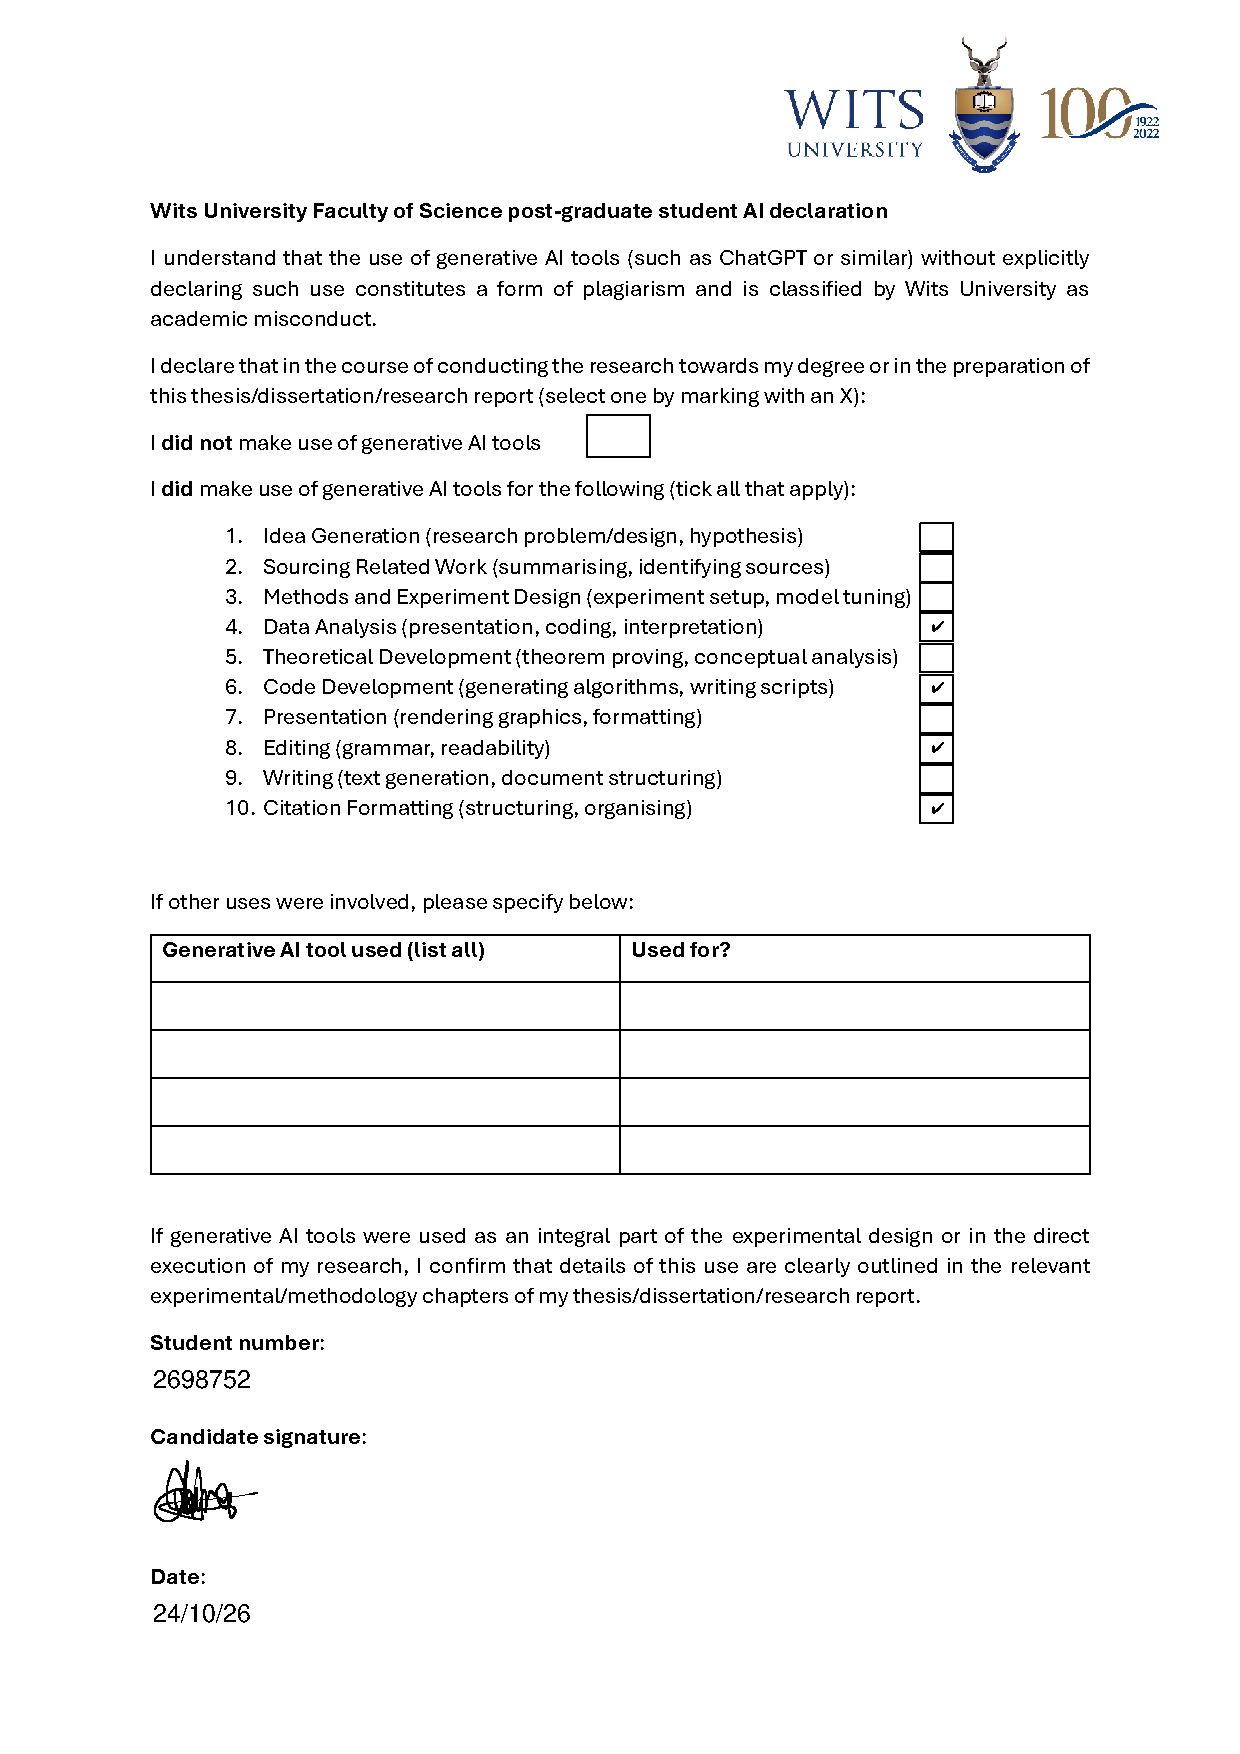
\includepdf[pages=-,pagecommand={\thispagestyle{empty}}]{ai_declaration.pdf}
\clearpage
\section*{Supplementary material}
\footnotesize
\subsection*{S1. Concepts, stems and the word forms they match (1 Nov 1884--1888, both papers)}
Stems are matched as substrings of surface forms; following \citet{schoots2023b} we inspected forms for false positives (our first \emph{law} stem also matched \emph{inteto}, speech, and was dropped) but did not hand-filter them, so run-together forms (e.g. \emph{rulumenteningomsebenzi}) and missed variants remain. All stems, forms and glosses await review by a first-language isiXhosa speaker; e.g.\ \emph{rulumente} is glossed `government' here but `parliament' by Schoots et al.\ (2023a, p.~62). Political concepts were fixed before testing; religion was suggested by the classifier and is exploratory.\\[2pt]
\begin{tabular}{@{}p{1.9cm}p{1.6cm}p{2.0cm}p{9.6cm}@{}}
\toprule
Concept & Type & Stems & Most frequent matched forms (count; number of distinct forms) \\ \midrule
parliament & political & palamente & palamente (1754), ipalamente (47), palamenteni (22), epalamente (14), bapalamente (1), nepalamente (1), yepalamente (1); 11 forms \\
vote & political & voti & ivoti (301), voti (217), evotini (136), abavoti (98), ngevoti (55), levoti (22), nevoti (22); 115 forms \\
government & political & rulumente, rulumeni & rulumente (1882), rulumeni (1336), rulumenteni (7), urulumente (5), urulumeni (3), rulumenini (2), serulumente (1); 14 forms \\
rule & political & mbuso & zombuso (169), umbuso (76), mbuso (60), yombuso (42), kombuso (37), lombuso (28), kulombuso (23); 43 forms \\
law & political & mteto & umteto (724), lomteto (475), mteto (406), ngomteto (167), ngumteto (94), komteto (76), nomteto (76); 82 forms \\
rights & political & lungelo & amalungelo (315), ilungelo (288), lungelo (113), nelungelo (54), namalungelo (50), lilungelo (39), elilungelo (37); 115 forms \\
country & political & lizwe & lizwe (646), ilizwe (292), kwelilizwe (201), elilizwe (101), elizwe (96), belilizwe (76), yelilizwe (52); 78 forms \\
land & political & mhlaba & umhlaba (836), mhlaba (208), lomhlaba (156), nomhlaba (105), komhlaba (99), somhlaba (95), yomhlaba (94); 135 forms \\
freedom & political & kululek & inkululeko (27), kukululekile (24), ukululekile (13), ngenkululeko (10), abakululekileyo (8), nkululeko (8), nenkululeko (7); 92 forms \\
humanity & political & buntu & ubuntu (45), yobuntu (14), nobuntu (8), sobuntu (8), buntu (7), lobuntu (7), zobuntu (6); 29 forms \\
time & neutral & xesha & ixesha (787), ngexesha (364), xesha (298), amaxesha (243), lixesha (191), ngamaxesha (149), zamaxesha (114); 207 forms \\
house & neutral & ndlu & indlu (719), izindlu (328), kwindlu (276), ndlu (234), yendlu (227), ngendlu (133), nendlu (130); 193 forms \\
rain & neutral & mvula & imvula (267), mvula (31), yemvula (23), ezimvula (17), lemvula (16), yimvula (14), zimvula (10); 45 forms \\
cattle & neutral & nkomo & inkomo (555), zenkomo (258), nkomo (193), yenkomo (93), nenkomo (75), ngenkomo (35), lenkomo (33); 79 forms \\
religion & exploratory & tixo, kristu, krestu & tixo (684), kristu (207), krestu (118), makristu (7), kristukazi (7), makrestu (6), mkrestu (5); 32 forms \\
\bottomrule
\end{tabular}

\subsection*{S2. Secondary framing tests across settings}
Percentile of the observed shift among 2000 frequency-matched word sets, and one-sided $p$ (uncorrected). Jaccard = shift in a word's ten nearest neighbours (neighbour overlap; \citealp{gonen2020}). P+V = \emph{palamente} + \emph{voti}; P+V+R adds \emph{rulumente} (uncertain meaning). Directional $\Delta$: Isigidimi minus Imvo, religious minus political similarity (in $z$-score units), political concepts, two-sided $p$ against matched sets; the last columns give the control \emph{house}. Three settings survive Bonferroni over five ($p<0.01$): window 1, window 2, and window 2 with forms joined. Joining partly disjunctive forms (\emph{uku ba}) leaves the global profile gap unchanged. Matched sets are re-drawn for each test; without \emph{land} the pooled set is smaller, so lower power may contribute to the higher $p$.\\[2pt]
\begin{tabular}{@{}lcccccccccc@{}}
\toprule
Setting & P+V profile & P+V Jaccard & P+V+R profile & P+V+R Jaccard & $\Delta$ & $\Delta$ $p$ & $p$ w/o land & house $\Delta$ & house $p$ \\ \midrule
window 1 (tuned) & 92 ($p$=0.083) & 96 ($p$=0.039) & 92 ($p$=0.077) & 99 ($p$=0.007) & +0.68 & $<$0.001 & 0.010 & +1.08 & $<$0.001 \\
window 1, forms joined & 99 ($p$=0.010) & 95 ($p$=0.053) & 100 ($p$=0.001) & 100 ($p$=0.002) & +0.44 & 0.016 & 0.088 & +1.15 & $<$0.001 \\
window 2 & 86 ($p$=0.139) & 94 ($p$=0.061) & 90 ($p$=0.096) & 99 ($p$=0.010) & +0.76 & $<$0.001 & 0.045 & +1.34 & $<$0.001 \\
window 2, forms joined & 91 ($p$=0.094) & 98 ($p$=0.023) & 99 ($p$=0.011) & 100 ($p$=0.002) & +0.58 & 0.009 & 0.064 & +1.51 & $<$0.001 \\
window 5 & 62 ($p$=0.382) & 98 ($p$=0.016) & 81 ($p$=0.189) & 100 ($p$=0.002) & +0.66 & 0.015 & 0.256 & +0.84 & 0.061 \\
\bottomrule
\end{tabular}

\subsection*{S3. Era drift: does a concept's rate move across eras within one paper?}
Per-million-token rates and ratios (later/earlier, or Imvo/Isigidimi) with issue-bootstrap 95\% CIs.\\[2pt]
\begin{tabular}{@{}llrrl@{}}
\toprule
Concept & Comparison & First & Second & Ratio (95\% CI) \\ \midrule
parliament & Isigidimi: later / earlier era & 214 & 394 & 1.84 (0.96--4.98) \\
parliament & Imvo: later / earlier era & 1320 & 758 & 0.57 (0.50--0.66) \\
parliament & Imvo 1889-94 / Isigidimi 1876-83 (held-out) & 214 & 758 & 3.54 (1.98--9.58) \\
government & Isigidimi: later / earlier era & 2197 & 1095 & 0.50 (0.39--0.64) \\
government & Imvo: later / earlier era & 2234 & 1649 & 0.74 (0.67--0.81) \\
government & Imvo 1889-94 / Isigidimi 1876-83 (held-out) & 2197 & 1649 & 0.75 (0.65--0.88) \\
vote & Isigidimi: later / earlier era & 72 & 614 & 8.55 (3.51--18.94) \\
vote & Imvo: later / earlier era & 799 & 921 & 1.15 (0.88--1.51) \\
vote & Imvo 1889-94 / Isigidimi 1876-83 (held-out) & 72 & 921 & 12.82 (7.85--25.92) \\
religion & Isigidimi: later / earlier era & 2541 & 1678 & 0.66 (0.50--0.86) \\
religion & Imvo: later / earlier era & 445 & 612 & 1.38 (1.08--1.76) \\
religion & Imvo 1889-94 / Isigidimi 1876-83 (held-out) & 2541 & 612 & 0.24 (0.20--0.30) \\
\bottomrule
\end{tabular}

\subsection*{S4. Anchors for the directional test}
Anchors are the 15 top-PMI neighbours of each seed pair in held-out text (Isigidimi 1876-83 + Imvo 1889-94), frozen before testing. Religious (15 words; seeds \emph{tixo}, \emph{kristu}): \emph{sikelela}, \emph{sindisa}, \emph{ukumkanikazi}, \emph{inkosazana}, \emph{buka}, \emph{oyingcwele}, \emph{lilizwi}, \emph{msindisi}, \emph{nelizwi}, \emph{kwelizwi}, \emph{wanga}, \emph{lika}, \emph{yesu}, \emph{izono}, \emph{yehova}. Political (15 words; seeds \emph{palamente}, \emph{voti}): \emph{emqulwini}, \emph{wonyulo}, \emph{lonyulo}, \emph{elugqatsweni}, \emph{eziqingata}, \emph{lokunyula}, \emph{kwesase}, \emph{lokuvota}, \emph{endlu}, \emph{kwamagama}, \emph{ukumela}, \emph{izayo}, \emph{ngalomteto}, \emph{nawupina}, \emph{kwabase}. Seed words cannot themselves be tested (Fig.~S1). Political anchors include \emph{endlu} (`in the house'), which might have favoured the neutral control \emph{house}; re-running without \emph{endlu} leaves both the political lean and \emph{house}'s lean in place (outputs/framing\_matched\_tests\_noendlu.csv), and \emph{ngalomteto}, which contains the \emph{law} stem. Glosses are unverified: two religious anchors (\emph{ukumkanikazi}, \emph{inkosazana}) may reflect royal rather than religious register, and several anchors on both sides (\emph{lika}, \emph{buka}; \emph{nawupina}, \emph{kwabase}, \emph{izayo}) may be grammatical rather than topical, consistent with narrow-window PMI capturing grammar. All await speaker review.
\normalsize

\subsection*{S5. Readers' letters versus the rest of each paper}
Letters are detected by src/12\_letters.py: a letter opens by addressing the editor (vocative \emph{mhleli} or \emph{mcokeli}, not \emph{u/ku/ngu mhleli}, which refer to him) or by asking for insertion (\emph{ndifakele}, \emph{kaundifakele}), and ends at the signature (a run of very short lines). A hand check of 30 random detections found 28 genuine letters; the errors were usifake umkala (horse advert: `put a bit on it'); no mhleli wepepa lama bhulu ('and the editor of the Boer paper'). Recall was not measured. Imvo is restricted to the months in which Isigidimi has text; CIs from 4000 issue resamples; rates are not tested against matched sets. Hits = concept uses.\\[2pt]
\begin{tabular}{@{}llrrrrrr@{}}
\toprule
Part & Concept & Isig.\ tokens & Isig.\ hits & Imvo tokens & Imvo hits & Imvo/Isig. & 95\% CI \\ \midrule
letters & parliament & 18,344 & 2 & 70,475 & 48 & 6.25 & 2.09--16.92 \\
letters & religion & 18,344 & 57 & 70,475 & 77 & 0.35 & 0.19--0.69 \\
letters & vote & 18,344 & 4 & 70,475 & 58 & 3.77 & 1.04--18.93 \\
letters & government & 18,344 & 13 & 70,475 & 161 & 3.22 & 1.67--9.62 \\
rest of paper & parliament & 268,319 & 111 & 936,998 & 1280 & 3.30 & 2.53--4.51 \\
rest of paper & religion & 268,319 & 424 & 936,998 & 370 & 0.25 & 0.17--0.37 \\
rest of paper & vote & 268,319 & 172 & 936,998 & 821 & 1.37 & 0.79--2.83 \\
rest of paper & government & 268,319 & 301 & 936,998 & 1906 & 1.81 & 1.47--2.28 \\
\bottomrule
\end{tabular}

\subsection*{S6. Which sense of \emph{umhlaba}?}
For every use of the land stem (\emph{mhlaba}) we look at the 10 tokens either side. Religious cues: \emph{izulu}, \emph{lizulu}, \emph{nezulu}, and words containing \emph{zulwini}, \emph{tixo}, \emph{kristu}, \emph{yesu}, \emph{msindisi}, \emph{ngcwele} (bare \emph{zulu} is excluded: \emph{kwa zulu} is Zululand). Property/political cues: words containing \emph{taitile}, \emph{mteto}, \emph{rulumente}, \emph{palamente}, \emph{mantyi}, \emph{fama}, \emph{voti}, \emph{nyulo}, \emph{rafu}, \emph{lokishi}. Most uses have neither cue. Example lines for a speaker to check are in outputs/land\_kwic.md.\\[2pt]
\begin{tabular}{@{}llrrr@{}}
\toprule
Paper & Cue & Uses & Share & 95\% CI \\ \midrule
Imvo & religious & 1408 & 0.9\% & 0.4--1.4\% \\
Imvo & property/political & 1408 & 26.8\% & 23.8--29.7\% \\
Isigidimi & religious & 353 & 3.4\% & 1.7--5.3\% \\
Isigidimi & property/political & 353 & 12.7\% & 8.5--17.7\% \\
\bottomrule
\end{tabular}

\subsection*{S7. Same editor, different control; same control, different editor}
Cells (editors after Schoots, 2023b, p.~71): Jabavu edits Isigidimi (Jan 1881--Oct 1884); Jabavu edits Imvo (Nov 1884--1888); Gqoba edits Isigidimi (Nov 1884--1888); Makiwane edits Isigidimi (1876--80; Stewart until 1876). Ratios of rates per million tokens; 95\% CIs from 4000 issue resamples; $p$: two-sided, against 2000 matched sets of random words (src/15\_editor\_control.py). Every contrast is also a contrast in time; \emph{rule} has only 9 uses in Jabavu's Isigidimi, so its large ratios are not interpreted.\\[2pt]
\begin{tabular}{@{}lrrrrrrrrr@{}}
\toprule
Concept & \multicolumn{3}{c}{Jabavu: Imvo / Isigidimi} & \multicolumn{3}{c}{Isigidimi: Gqoba / Jabavu} & \multicolumn{3}{c}{Isigidimi: 1881--84 / 1876--80} \\
 & ratio & 95\% CI & $p$ & ratio & 95\% CI & $p$ & ratio & 95\% CI & $p$ \\ \midrule
parliament & 1.69 & 1.23--2.54 & 0.088 & 0.50 & 0.33--0.79 & 0.043 & 49.86 & 14.41--405.79 & $<$0.001 \\
vote & 3.07 & 1.98--5.23 & 0.017 & 2.36 & 1.07--4.61 & 0.034 & 11.63 & 4.32--98.99 & 0.004 \\
government & 1.21 & 0.99--1.49 & 0.387 & 0.59 & 0.44--0.77 & 0.043 & 0.78 & 0.61--1.01 & 0.289 \\
rule & 19.47 & 9.46--77.40 & 0.001 & 8.28 & 3.57--31.56 & 0.009 & 0.38 & 0.09--1.32 & 0.228 \\
law & 1.36 & 1.08--1.72 & 0.235 & 0.80 & 0.53--1.17 & 0.376 & 1.31 & 0.98--1.76 & 0.314 \\
rights & 0.93 & 0.76--1.16 & 0.808 & 0.82 & 0.58--1.13 & 0.480 & 2.91 & 2.05--4.12 & 0.006 \\
country & 1.08 & 0.92--1.29 & 0.773 & 1.13 & 0.90--1.41 & 0.596 & 0.74 & 0.59--0.92 & 0.243 \\
land & 1.10 & 0.91--1.34 & 0.689 & 0.95 & 0.70--1.28 & 0.853 & 0.94 & 0.76--1.16 & 0.815 \\
freedom & 0.68 & 0.51--0.92 & 0.443 & 0.95 & 0.64--1.38 & 0.899 & 1.52 & 1.01--2.42 & 0.408 \\
humanity & 0.97 & 0.59--1.90 & 0.959 & 1.88 & 0.98--3.88 & 0.227 & 0.97 & 0.45--1.96 & 0.967 \\
religion & 0.37 & 0.27--0.50 & 0.025 & 1.38 & 1.03--1.83 & 0.168 & 0.35 & 0.26--0.47 & $<$0.001 \\
\bottomrule
\end{tabular}

\subsection*{S8. Hyper-parameter search for the embeddings}
fastText skip-gram, tuned on text outside the test window (Isigidimi 1876--83, Imvo 1889--94) so that tuning never sees the compared years. Criterion: seed stability, the mean top-10 nearest-neighbour overlap between two runs that differ only in random seed \citep{antoniak2018}; unstable embeddings would turn noise into apparent shifts. 34 settings over dimension (50, 100, 200, 300, 400), window (1, 2, 3, 5, 8) and epochs (10, 20, 30), searched in rounds that extended the grid past each optimum. Chosen: dimension 400, window 1, 20 epochs. Stability is highest at the narrowest window, which favours grammar over topic; the paper therefore also reports windows 2 and 5 (Table S2). Best setting per window:\\[2pt]
\begin{tabular}{@{}rrrrrr@{}}
\toprule
Window & Dimension & Epochs & Isigidimi 1876--83 & Imvo 1889--94 & Mean stability \\ \midrule
1 & 400 & 20 & 0.844 & 0.814 & 0.829 \\
2 & 300 & 20 & 0.823 & 0.798 & 0.810 \\
3 & 300 & 20 & 0.810 & 0.799 & 0.805 \\
5 & 400 & 20 & 0.798 & 0.796 & 0.797 \\
8 & 200 & 10 & 0.758 & 0.755 & 0.757 \\
\bottomrule
\end{tabular}\\[2pt]
At the chosen setting, word2vec reaches a stability of 0.64 against fastText's 0.83, so fastText is used throughout.

\subsection*{S9. Tokenizer cost}
Each condition is a random sample of about 100{,}000 words. Modern text is the isiXhosa section of MasakhaNEWS \citep{adelani2023}. The old-spelling condition is the same modern sample with the aspiration marks of modern orthography removed by fixed rules (\emph{th}$\to$\emph{t}, \emph{kh}$\to$\emph{k}, \emph{ph}$\to$\emph{p}, \emph{rh}$\to$\emph{r}, \emph{ch}$\to$\emph{c}, \emph{qh}$\to$\emph{q}, \emph{xh}$\to$\emph{x}; src/05\_fertility.py), so only spelling changes and the words stay the same: it is compared per word. Historical text differs in word division, so it is compared per 100 characters. The politics/business sample checks genre within modern news: its cost is close to all modern news, while both 1880s papers cost more, so the historical penalty is not simply a news-topic effect, though 1880s and modern newspapers still differ in genre. 95\% CIs from bootstrap resampling are within $\pm$0.01 subwords per word.\\[2pt]
\begin{tabular}{@{}lrrrrrrr@{}}
\toprule
Condition & Words & \multicolumn{2}{c}{XLM-R} & \multicolumn{2}{c}{Serengeti} & \multicolumn{2}{c}{mBERT} \\
 & & per word & per 100 ch. & per word & per 100 ch. & per word & per 100 ch. \\ \midrule
Modern news & 100,003 & 2.613 & 35.28 & 1.867 & 25.21 & 3.040 & 41.05 \\
Modern news, old spelling & 100,003 & 2.555 & 35.56 & 1.909 & 26.57 & 2.937 & 40.88 \\
Modern news, politics/business only & 88,389 & 2.673 & 35.21 & 1.888 & 24.88 & 3.116 & 41.06 \\
Isigidimi 1884--88 & 100,013 & 2.259 & 36.71 & 1.743 & 28.33 & 2.569 & 41.75 \\
Imvo 1884--88 (matched draw) & 100,006 & 2.240 & 36.92 & 1.738 & 28.65 & 2.533 & 41.75 \\
\bottomrule
\end{tabular}

\renewcommand{\thefigure}{S\arabic{figure}}\setcounter{figure}{0}
\begin{figure}[h]\centering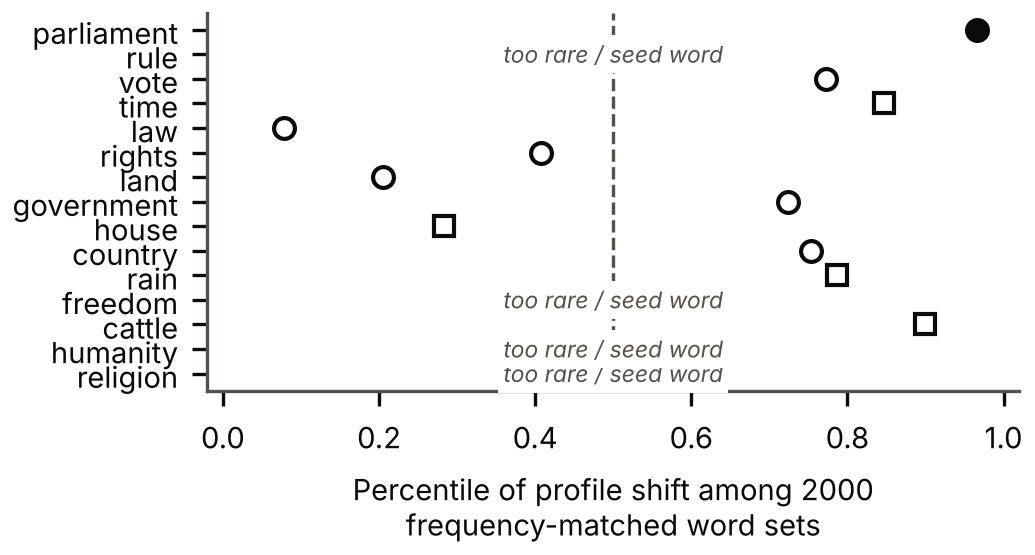
\includegraphics[width=3.45in]{fig_framing.png}
\caption{Profile-shift percentile of each concept among matched sets (markers as in Fig.~1, left); `too rare' = too few occurrences, `seed word' = anchor source, untestable.}\end{figure}
\begin{figure}[h]\centering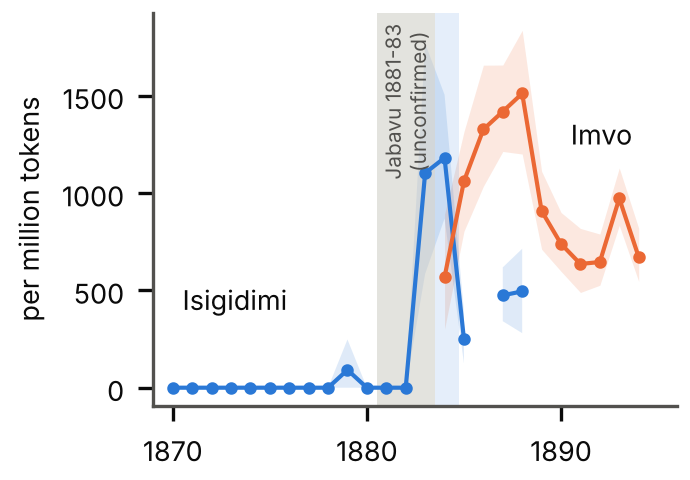
\includegraphics[width=2.3in]{fig_parliament_by_year.png}
\caption{Parliamentary vocabulary per million tokens; it enters Isigidimi in 1883 (light blue: twice-monthly issues, Schoots et al., 2023a, p.~59).}\end{figure}

\end{document}
